\documentclass[VM.tex]{subfiles}
\tikzset{
  load/.style   = {ultra thick,-latex},
  stress/.style = {-latex},
  dim/.style    = {latex-latex},
  axis/.style   = {-latex,black!55},
}

% Drawing View
\tikzset{dimetric2/.style={
  x={(0.935cm,-0.28cm)},
  y={(0.44cm, 0.312cm)},
  z={(0.000cm, 0.943cm)},
}}
\begin{document}

\subsubsection*{Description : }
A simply Supported square plate with distributed load (q). 
\subsubsection*{Reference : }
S.Timoshenko , S . Woinowsky , Theory of Plates and Shells , pg:381, Article : 30 . \\

\subsubsection*{Material and Geometric data : }


\begin{figure}[h!]
\centering
\subfile{TIM381_DRAW.tex}
\caption{TIM381} \label{TIM381sch}
\end{figure}
\begin{table}[h!]
\renewcommand{\arraystretch}{1.5}
\centering
\caption{Input Data}
\label{my-labelsdqf}
\begin{tabular}{|ll|ll|ll|}
\hline
\multicolumn{2}{|l|}{\cellcolor[HTML]{C0C0C0}Material Property} & \multicolumn{2}{l|}{\cellcolor[HTML]{C0C0C0}Geometric Data} & \multicolumn{2}{l|}{\cellcolor[HTML]{C0C0C0}Loading Data} \\ \hline  \hline
Young's Modulus ($E$)          & 2E11 $pa$         & Length ($a$)        & 10 $m$        &      Axial Tension($N_x$) & 2E7 $N/m$      \\
Poission's Ratio ($\nu$)       & 0.3         & Breath ($b$)        & 10 $m$          & Distributed Load ($q$)        & 1000 $N/m^2$       \\ 
    &         & Thickness($t$)        & 0.1 $m$          &    &        \\ \hline
\end{tabular}
\end{table}




\subsubsection*{Mesh and boundary condition : }



\begin{figure}[h!]
\begin{subfigure}{.45\textwidth}
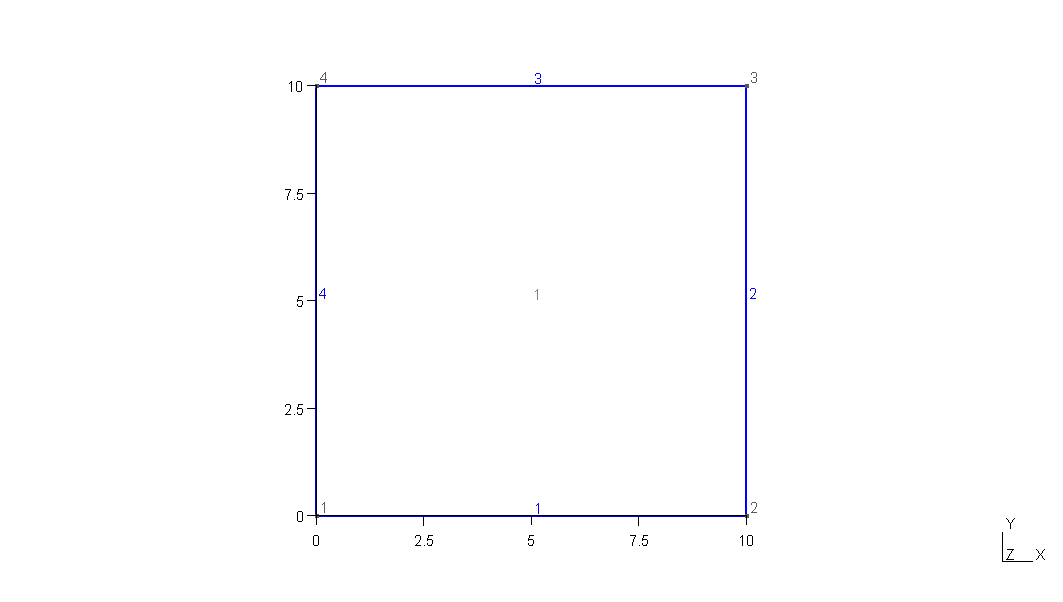
\includegraphics[width=\linewidth,trim={8cm 0 8cm 0},clip]{TIM381/TIM381_geo.png}
%\caption{Mode Shape 4}
\end{subfigure} \hfill
\begin{subfigure}{.45\textwidth}
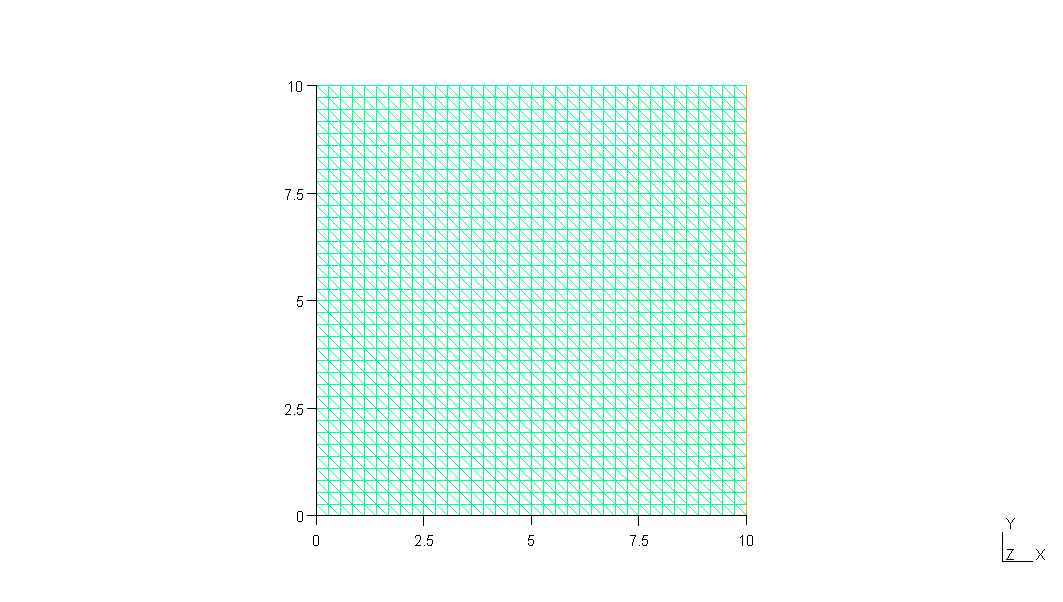
\includegraphics[width=\linewidth,trim={8cm 0 8cm 0},clip]{TIM381/TIM381_msh.png}
%\caption{Mode Shape 5}
\end{subfigure}
\caption{Geomentry and Mesh of TIM381}
\end{figure}







\begin{table}[h!]
\renewcommand{\arraystretch}{1.5}
\centering
\caption{FEM and Boundary condition data}
\label{my-label}
\begin{tabular}{|l|lll|l|lll|}
\hline
 \multicolumn{4}{l|}{\cellcolor[HTML]{C0C0C0}Direchlet Boundary} & \multicolumn{4}{l|}{\cellcolor[HTML]{C0C0C0}Neumann Boundary} \\ \hline \hline
Geo - \newline Entity      & $w$          & $\theta _ x$     & $\theta _ y $    & Geo - \newline Entity         & $F_z$        & $M_x$        & $M_y$        \\    
                 line \{1,2,3,4\}                   & Fixed      & Free         & Free        & Area \{1\}                    & 1000 $N/m^2$        &           &           \\ \hline & & & & Geo - \newline Entity         & Fx & &     
\\ \ & & & & line\{1,3\} & 2E7 $N/m$ & &

 \\ \hline
\end{tabular}
\end{table}
\subsubsection*{Analytically solution : }
The $w_{max}$which is the w displacement at the middle of the plate is given by
\begin{equation}
w_{max}=\alpha \frac{qb^4}{E t ^ 3}
\end{equation}
Where $\alpha$ can be taken from the graph given in the figure : \ref{fig:graph}. For this problem alpha is taken as $\alpha \approx 0.0113 $.
\begin{wrapfigure}{r}{0.5\textwidth}
\begin{center}
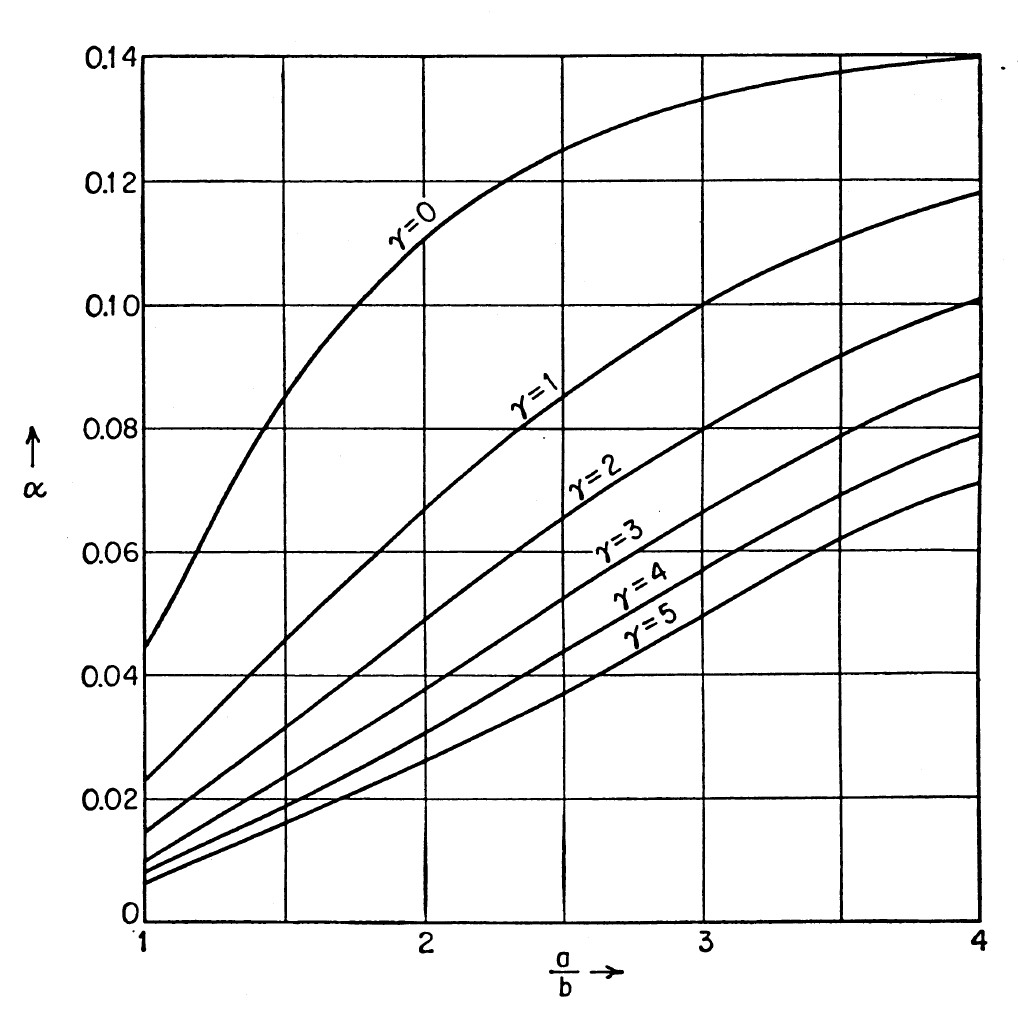
\includegraphics[width=0.45\textwidth]{TIM381/graph.png}
\end{center}
\caption{Graph to find $\alpha$ . }
\label{fig:graph}
\end{wrapfigure}

The parameter $\gamma$ is given by 
\begin{equation}
\gamma = \frac{N_xb^2}{4\pi^2D}
\end{equation}
The analytically solution of the problem is calculated as $w_{max} =0.000565m $

\subsubsection*{Result and error analysis : }

\begin{figure}[h!]
\centering
\minipage{1\textwidth}%
  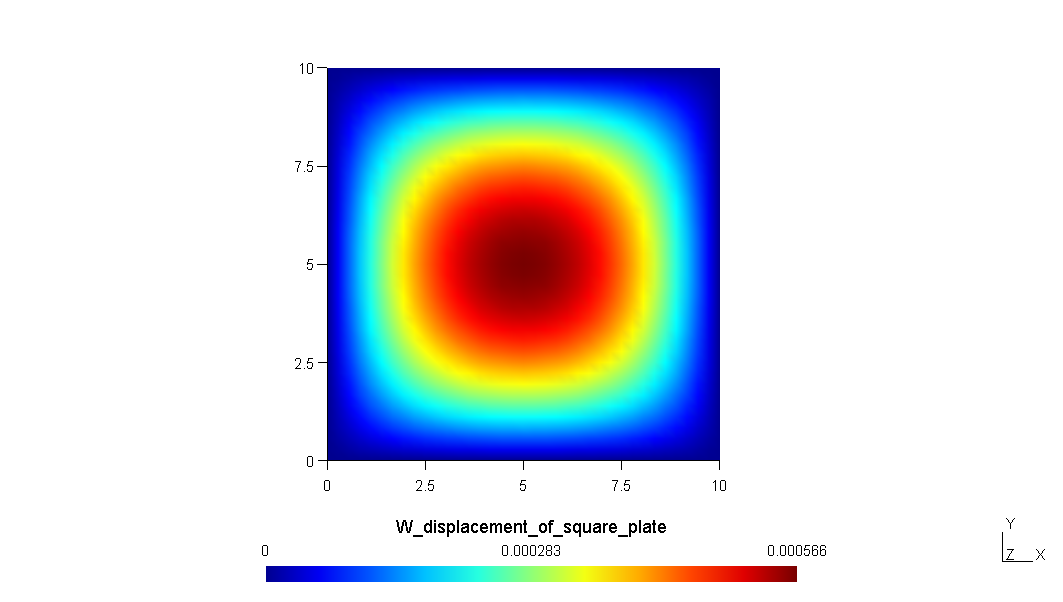
\includegraphics[width=\linewidth,trim={8cm 0 8cm 0},clip]{TIM381/TIM381_pos.png}
  \caption{FEM solution plot}\label{fig:awesome_image3}
\endminipage
\end{figure}
The maximum displacement of the domain is our solution . w displacement at middle is $ 0.000566 m $.


So the Error percentage is $ 0.17 \% $. 
\vspace{5cm}

\end{document}